% !TEX root = ../../thesis.tex

\cleartoleftpage
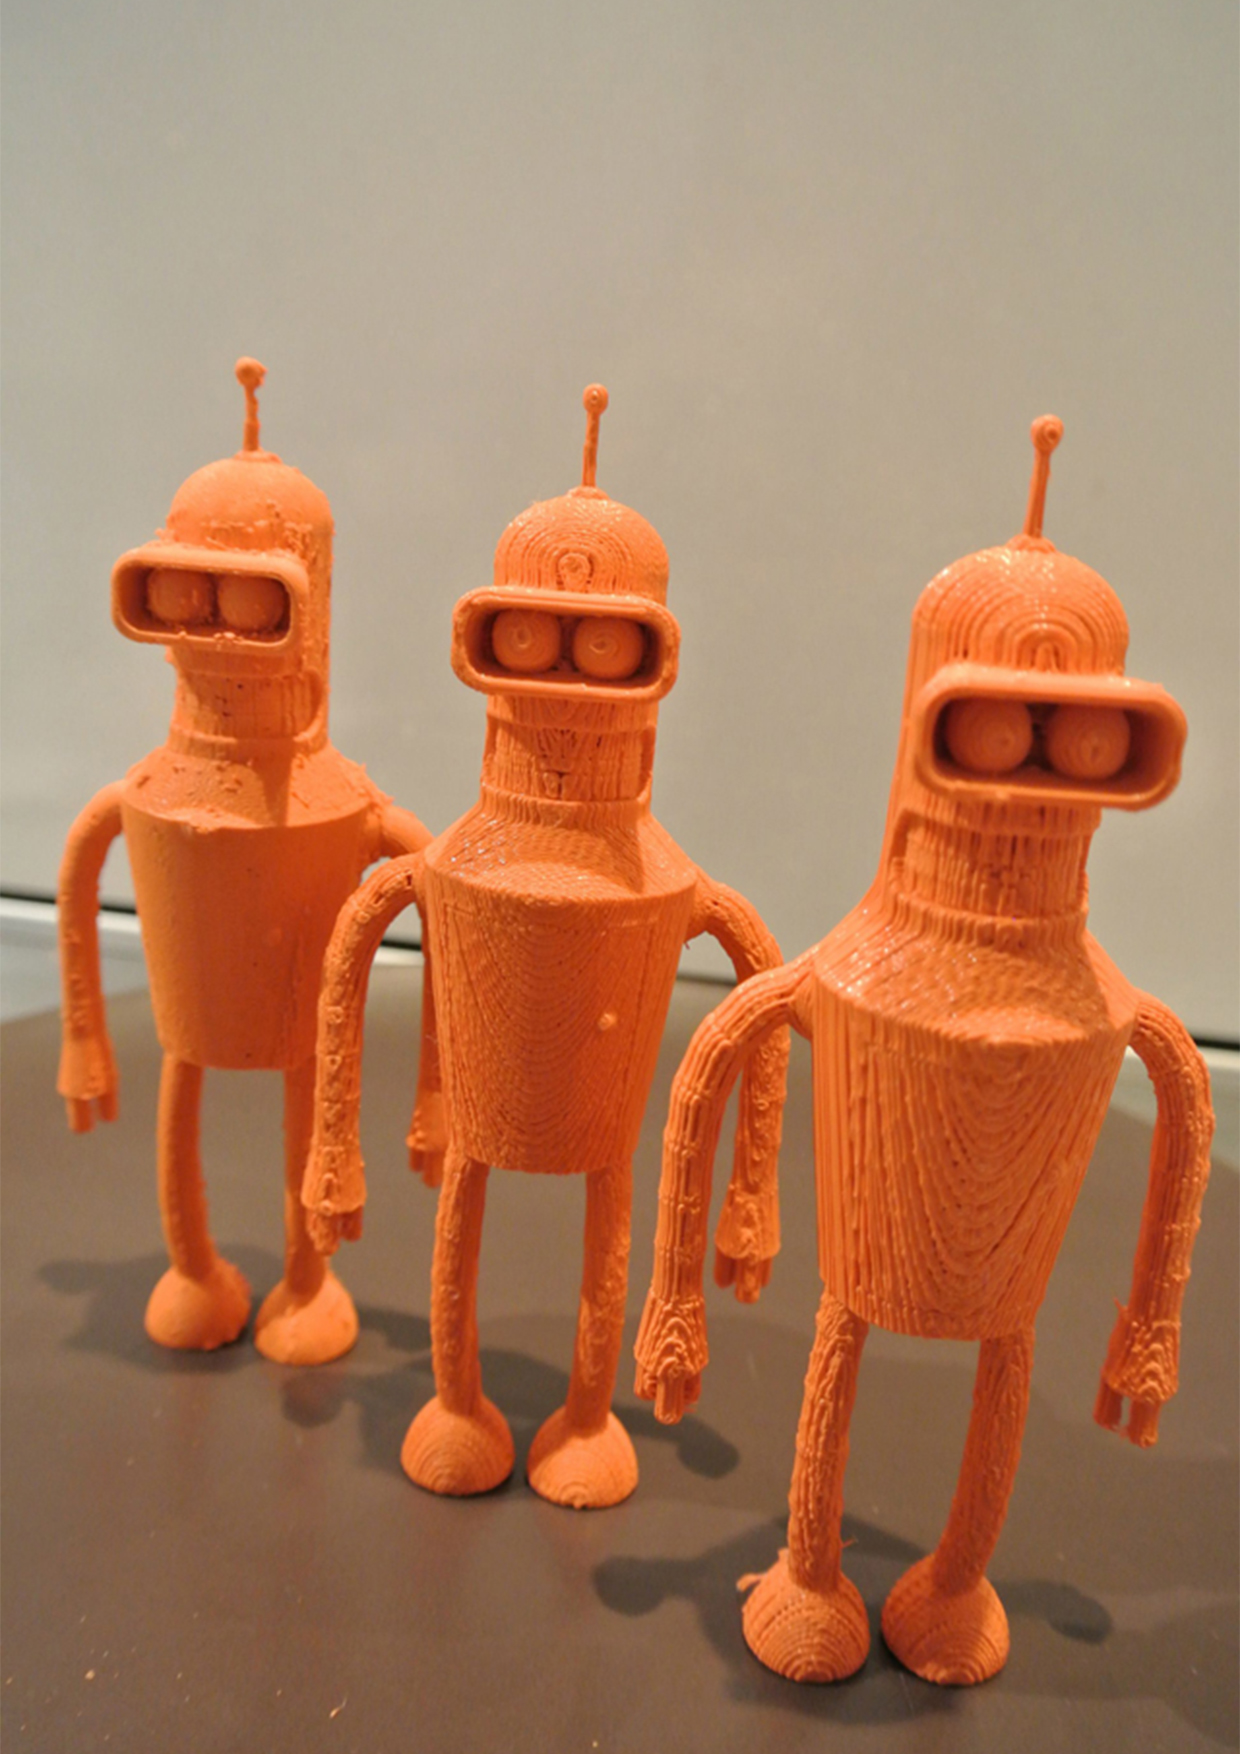
\includepdf{../media/chapter_illustration/3DprintedBlender.pdf}

\chapter{The open hardware and 3D printing revolution}

% \cleanchapterquote{third industrial revolution}{the economist}


\section{Introduction} % (fold)

With the democratization of personal computers and the development of Internet, computer science and relative applications have know a great expansion. Open source software played a major role, indeed most of the web server are running under Linux operating system and Apache while open source software like WordPress, Qt, Firefox, VLC and so on permitted the realization of a wide variety of daily life applications~\cite{peeling2001analysis}.

However while copying and sharing bits of a software is virtually free and can often be run on any computer, producing the atoms of a real object both has a potentially high cost and requires expert tooling. Thus the production of mechanic or electronic hardware components is limited to two options: either it is handcrafted or mass produced. Also the step between handcrafted prototype and mass production is so high only big company can reach it. Conventional manufacturing processes requires the production of specific tools, the programming of complex machine, the human intervention to put the part along the different tool and so on, most of the cost are in the up-front tooling, and the more complicated a product is, the more it costs. Thus, most of companies will not accept to run a whole production process just for few units and if they accept the cost will be so high than most prototypes never find a way to reach people outside the workshop they had been created. So until now, production in small or medium series has been extremely difficult to achieve because it was not profitable.
Only big companies were able to raise enough money to produce new hardware leading the niche products and personalization left aside.

Since few years, a novel evolution is going to completely change the current rules of the production and distribution of goods. This evolution is acting on both technological and political/societal aspects which tends to confirm those who argue it will be the next industrial revolution~\cite{anderson}. Indeed, new rapid prototyping technologies are emerging and make the production both cheap, fast and easy to anyone. At the same time the associated machines and tools are diffused under open source hardware licenses acting as a unexpected lever arm toward the diffusion of such technologies to anyone. All these radical changes are contextualized by the phenomenon of \emph{makers} and the exponential growth of associative production places (e.g Fab Lab, Makerspace, Tech Shop or Hackerspace).

In this chapter, we will first present and discuss the groundbreaking 3D printing technology. Then we will present the open source hardware movement and how its interaction with 3D printing is changing the current production paradigm.


\section{The 3D printing revolution} % (fold)

Prototyping is an essential step in a product development and manufacturing cycle. It permits to test the form and the functionalities of a new product before large investment in tooling for mass production. Until the last decade, prototypes were largely handmade by skilled craftsmen, adding weeks or months to the product development time.

The 3D printing is any of various processes of making a three-dimensional object from a digital model primarily through additive processes in which successive layers of material are laid down under computer control.
It permits to produce accurate parts right from a numeric model in few hours and with minimum handling tasks. Consequently, errors are minimized and product development costs and lead times substantially reduced. It has been claimed that rapid prototyping can cut new product costs by up to 70\% and the time to market by 90\%~\cite{waterman1994rapid}.

The last progress in the 3D printing process allow now to not only consider the 3D printing as a way to produce prototype but also as an actual production technique. Indeed the layered method of assembly allows intricate designs - geometries which are either impossible or too expensive to achieve with conventional metal casting (see \figurename~\ref{fig:3D_printed_objects}).


\begin{figure}[!b]
\centering
    \subfloat[][Nylon]{\label{fig:3Dprinted_part}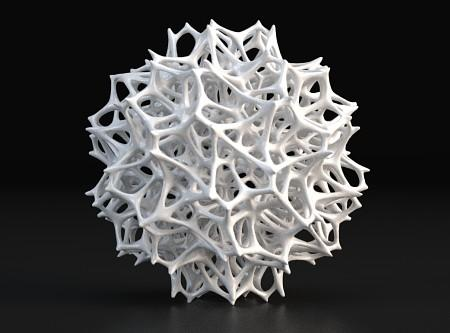
\includegraphics[height=3.5cm]{complex_3Dprinted_part.jpeg}}
    \hfil
    \subfloat[][Steel]{\label{fig:3Dprinted_steel}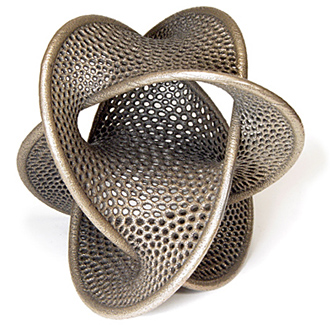
\includegraphics[height=3.5cm]{complex_3Dprint_steel.jpg}}
    \hfil
    \subfloat[][Odd Guitar]{\label{fig:3Dprinted_guitar}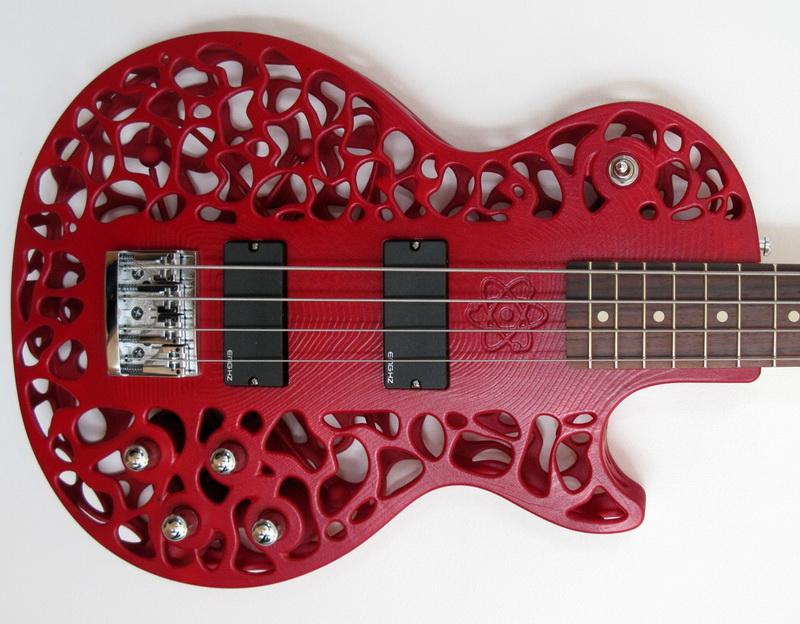
\includegraphics[height=3.5cm]{3D_printed_odd_guitar.jpg}}
    \caption{Some example of 3D printed parts which were until now impossible to produce. In addition, it can be done large range of material from wax to titanium.}
    \label{fig:3D_printed_objects}
\end{figure}

In this section we details the different 3D printing techniques available with pros and cons, then we will discuss the expected change in the industrial industry.

\subsection{Several techniques} % (fold)

The 3D printing name gather together several different additive processes.

\subsubsection{Fused Deposition Modeling (FDM)} % (fold)

The FDM technique relies on melting and selectively depositing a thin filament of thermoplastic polymer (ABS - PLA) in a cross-hatching fashion to form each layer of the part. The material is in the form of a wire supplied in sealed spools which is mounted on the machine and the wire is threaded through the FDM head. The head is moved in the horizontal X and Y directions for producing each layer through zigzag movements. The supporting table moves in the vertical direction and is lowered after the completion of each layer.

\begin{figure}[h]
    \centering
        \subfloat[][FDM process]{\label{fig:FDM_process}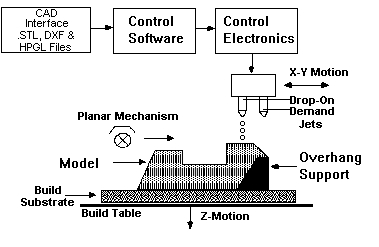
\includegraphics[height=4.5cm]{FDM_technique.jpg}}
        \hfil
        \subfloat[][FDM result example]{\label{fig:FDM_part}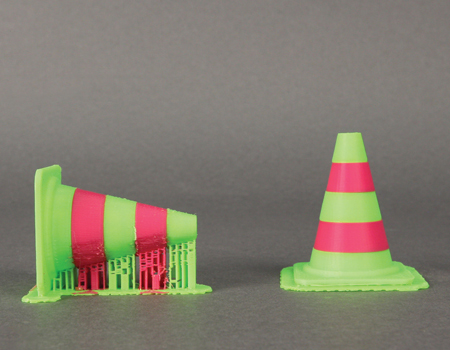
\includegraphics[height=4.5cm]{FDM_part.jpg}}
        \hfil
    \caption{}
    \label{fig:FDM_technique}
\end{figure}

It is a really low-cost and office environment friendly technique but is limited by its slowness on dense part, the need of supports and its lack of precision for details, thin walls and surface finish.


\subsubsection{Stereo-Lithography (SLA)} % (fold)

This technique relies on a photosensitive monomer resin which forms a polymer and solidifies when exposed to ultraviolet (UV) light. The UV laser beam moves in the horizontal directions and is focused on the top layer to polymerize the photo sensitive resin (see \figurename~\ref{fig:SLA_process}). Due to the absorption and scattering of the beam this reaction only takes place near the surface. Then the cured layer of polymer is lowered by the platform (Z axis) so that a fresj layer of liquid resin covers the part.

\begin{figure}[h]
    \centering
        \subfloat[][SLA process]{\label{fig:SLA_process}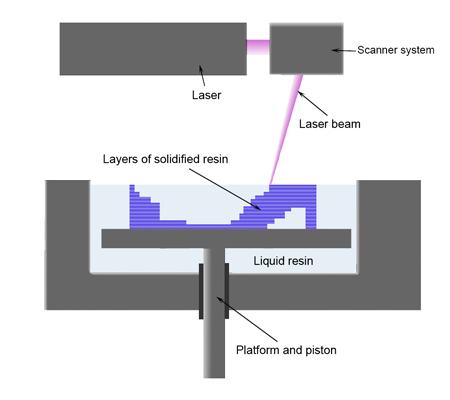
\includegraphics[height=5cm]{SLA_technique.jpg}}
        \hfil
        \subfloat[][SLA example]{\label{fig:formlab_printer}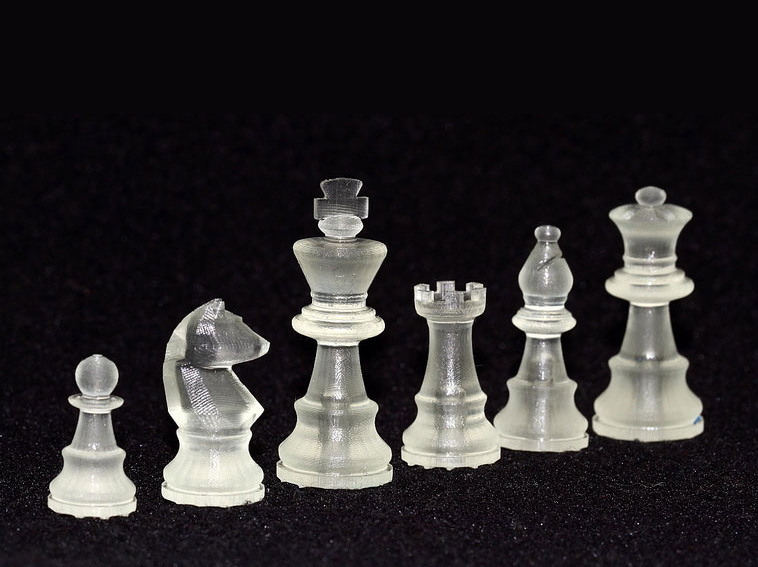
\includegraphics[height=5cm]{SLA_part.jpg}}
        \hfil
    \caption{The stereo-lithography technique: an UV laser beam polymerizes the top layer of a photo sensitive resin on the horizontal direction (X/Y) while the platform move in the vertical direction.}
    \label{fig:SLA_technique}
\end{figure}

This technique has several advantages such as a good surface finish and is capable to produce high detailed part with thin walls, but is limited by material (only photo polymers) and support structures are always needed which can be difficult to revome.

\subsubsection{Selective Laser Sintering (SLS)} % (fold)
The Selective Laser Sintering process uses a high power (25-50W) CO2 laser beam which melts and fuses fine powdered material spread on a layer. Before the powder is sintered, the entire bed is headted to just below the melting point of the material in order to minimize thermal distortion and facilitate fusion to the previous layer.
While the laser acts in the horizontal plane, the platform move along the vertical axis -through a distance corresponding to the layer thickness (usually 0.01 mm)- and a counter-rotating roller spreads a precise amount of fresh powder above the sintered layer. The unsintered powder serves as the support for overhanging portions, if any in the subsequent layers.

\begin{figure}[h]
    \centering
        \subfloat[][SLS process]{\label{fig:SLA_process}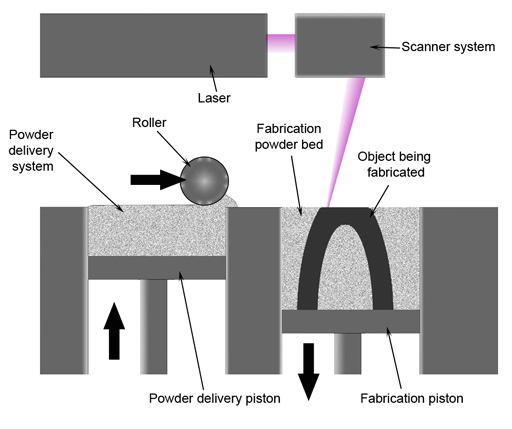
\includegraphics[height=5cm]{SLS_technique.jpg}}
        \hfil
        \subfloat[][]{\label{fig:formlab_printer}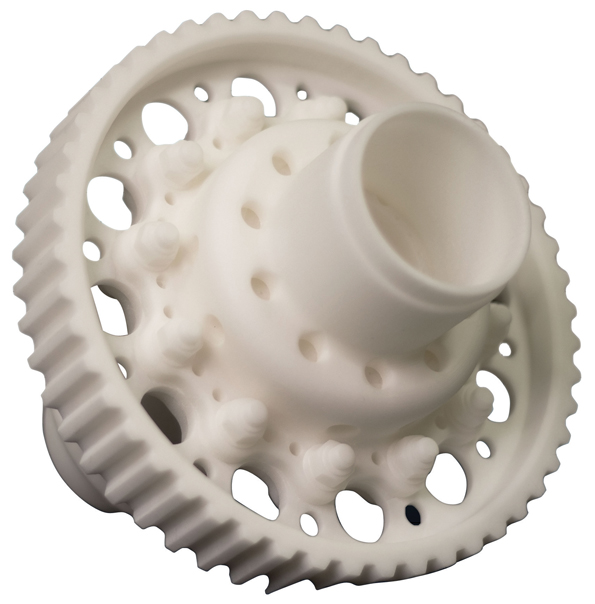
\includegraphics[height=5cm]{SLS_part.jpg}}
        \hfil
    \caption{}
    \label{fig:SLS_technique}
\end{figure}

This technique has really interesting advantage: it is compatible with a large number of different materials, it does not require support and mechanical properties of part are homegenous (the same in any direction). However, this technique requires some handling to extract extra powder from the part and SLS 3D printer are very expensive (+50K\$).


\subsubsection{Direct Metal Laser Sintering (DMLS)} % (fold)

The Direct Metal Laser Sintering is very similar with the SLS process but use a high-powered 200 watt Yb-fiber optic laser in order to fuse metal powder into a solid part by melting it locally. Parts are built up additively layer by layer, typically using layers 20 micrometres thick. This process allows for highly complex geometries to be created directly from the 3D CAD data, fully automatically, in hours and without any tooling. DMLS is a net-shape process, producing parts with high accuracy and detail resolution, good surface quality and excellent mechanical properties. However, this is obviously the most expensive technique.

\begin{figure}[h]
    \centering
        \subfloat[][DMLS part]{\label{fig:SLA_process}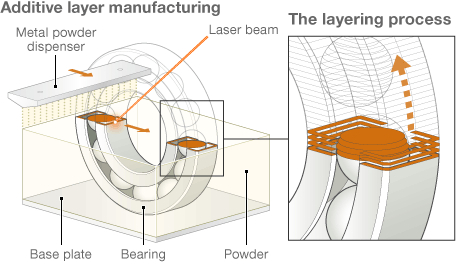
\includegraphics[height=4.5cm]{DMLS_technique.jpg}}
        \hfil
        \subfloat[][DMLS part]{\label{fig:SLA_process}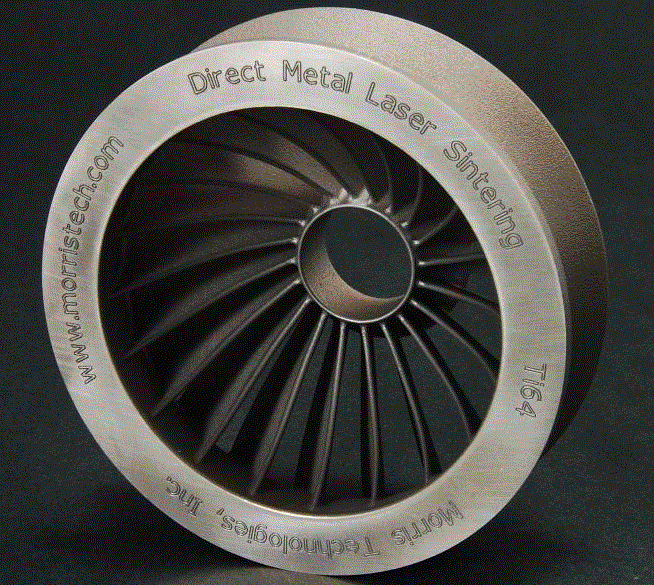
\includegraphics[height=4.5cm]{DMLS_part.jpg}}
        \hfil
    \caption{}
    \label{fig:DMLS_technique}
\end{figure}


\subsection{Expected major impact in the day to come} % (fold)

The 3D printing technique change the paradigm

As 3D printers became more accessible to consumers, online social platforms have developed to support the community.[131] This includes websites that allow users to access information such as how to build a 3D printer, as well as social forums that discuss how to improve 3D print quality and discuss 3D printing news, as well as social media websites that are dedicated to share 3D models.[132][133][134]
RepRap is a wiki based website that was created to hold all information on 3d printing, and has developed into a community that aims to bring 3D printing to everyone. Furthermore, there are other sites such as Thingiverse, which was created initially to allow users to post 3D files for anyone to print, allowing for decreased transaction cost of sharing 3D files. These websites have allowed for greater social interaction between users, creating communities dedicated around 3D printing.

At The University of Southern California, Professor Behrokh Khoshnevis has built a colossal 3D printer that can build a house in 24 hours. Khoshnevis's robot comes equipped with a nozzle that spews out concrete and can build a home based on a set computer pattern.



\begin{figure}[h]
\centering
    \subfloat[][SuperDraco rocket engine has a combustion chamber 3D printed - SpaceX.]{\label{fig:superdraco}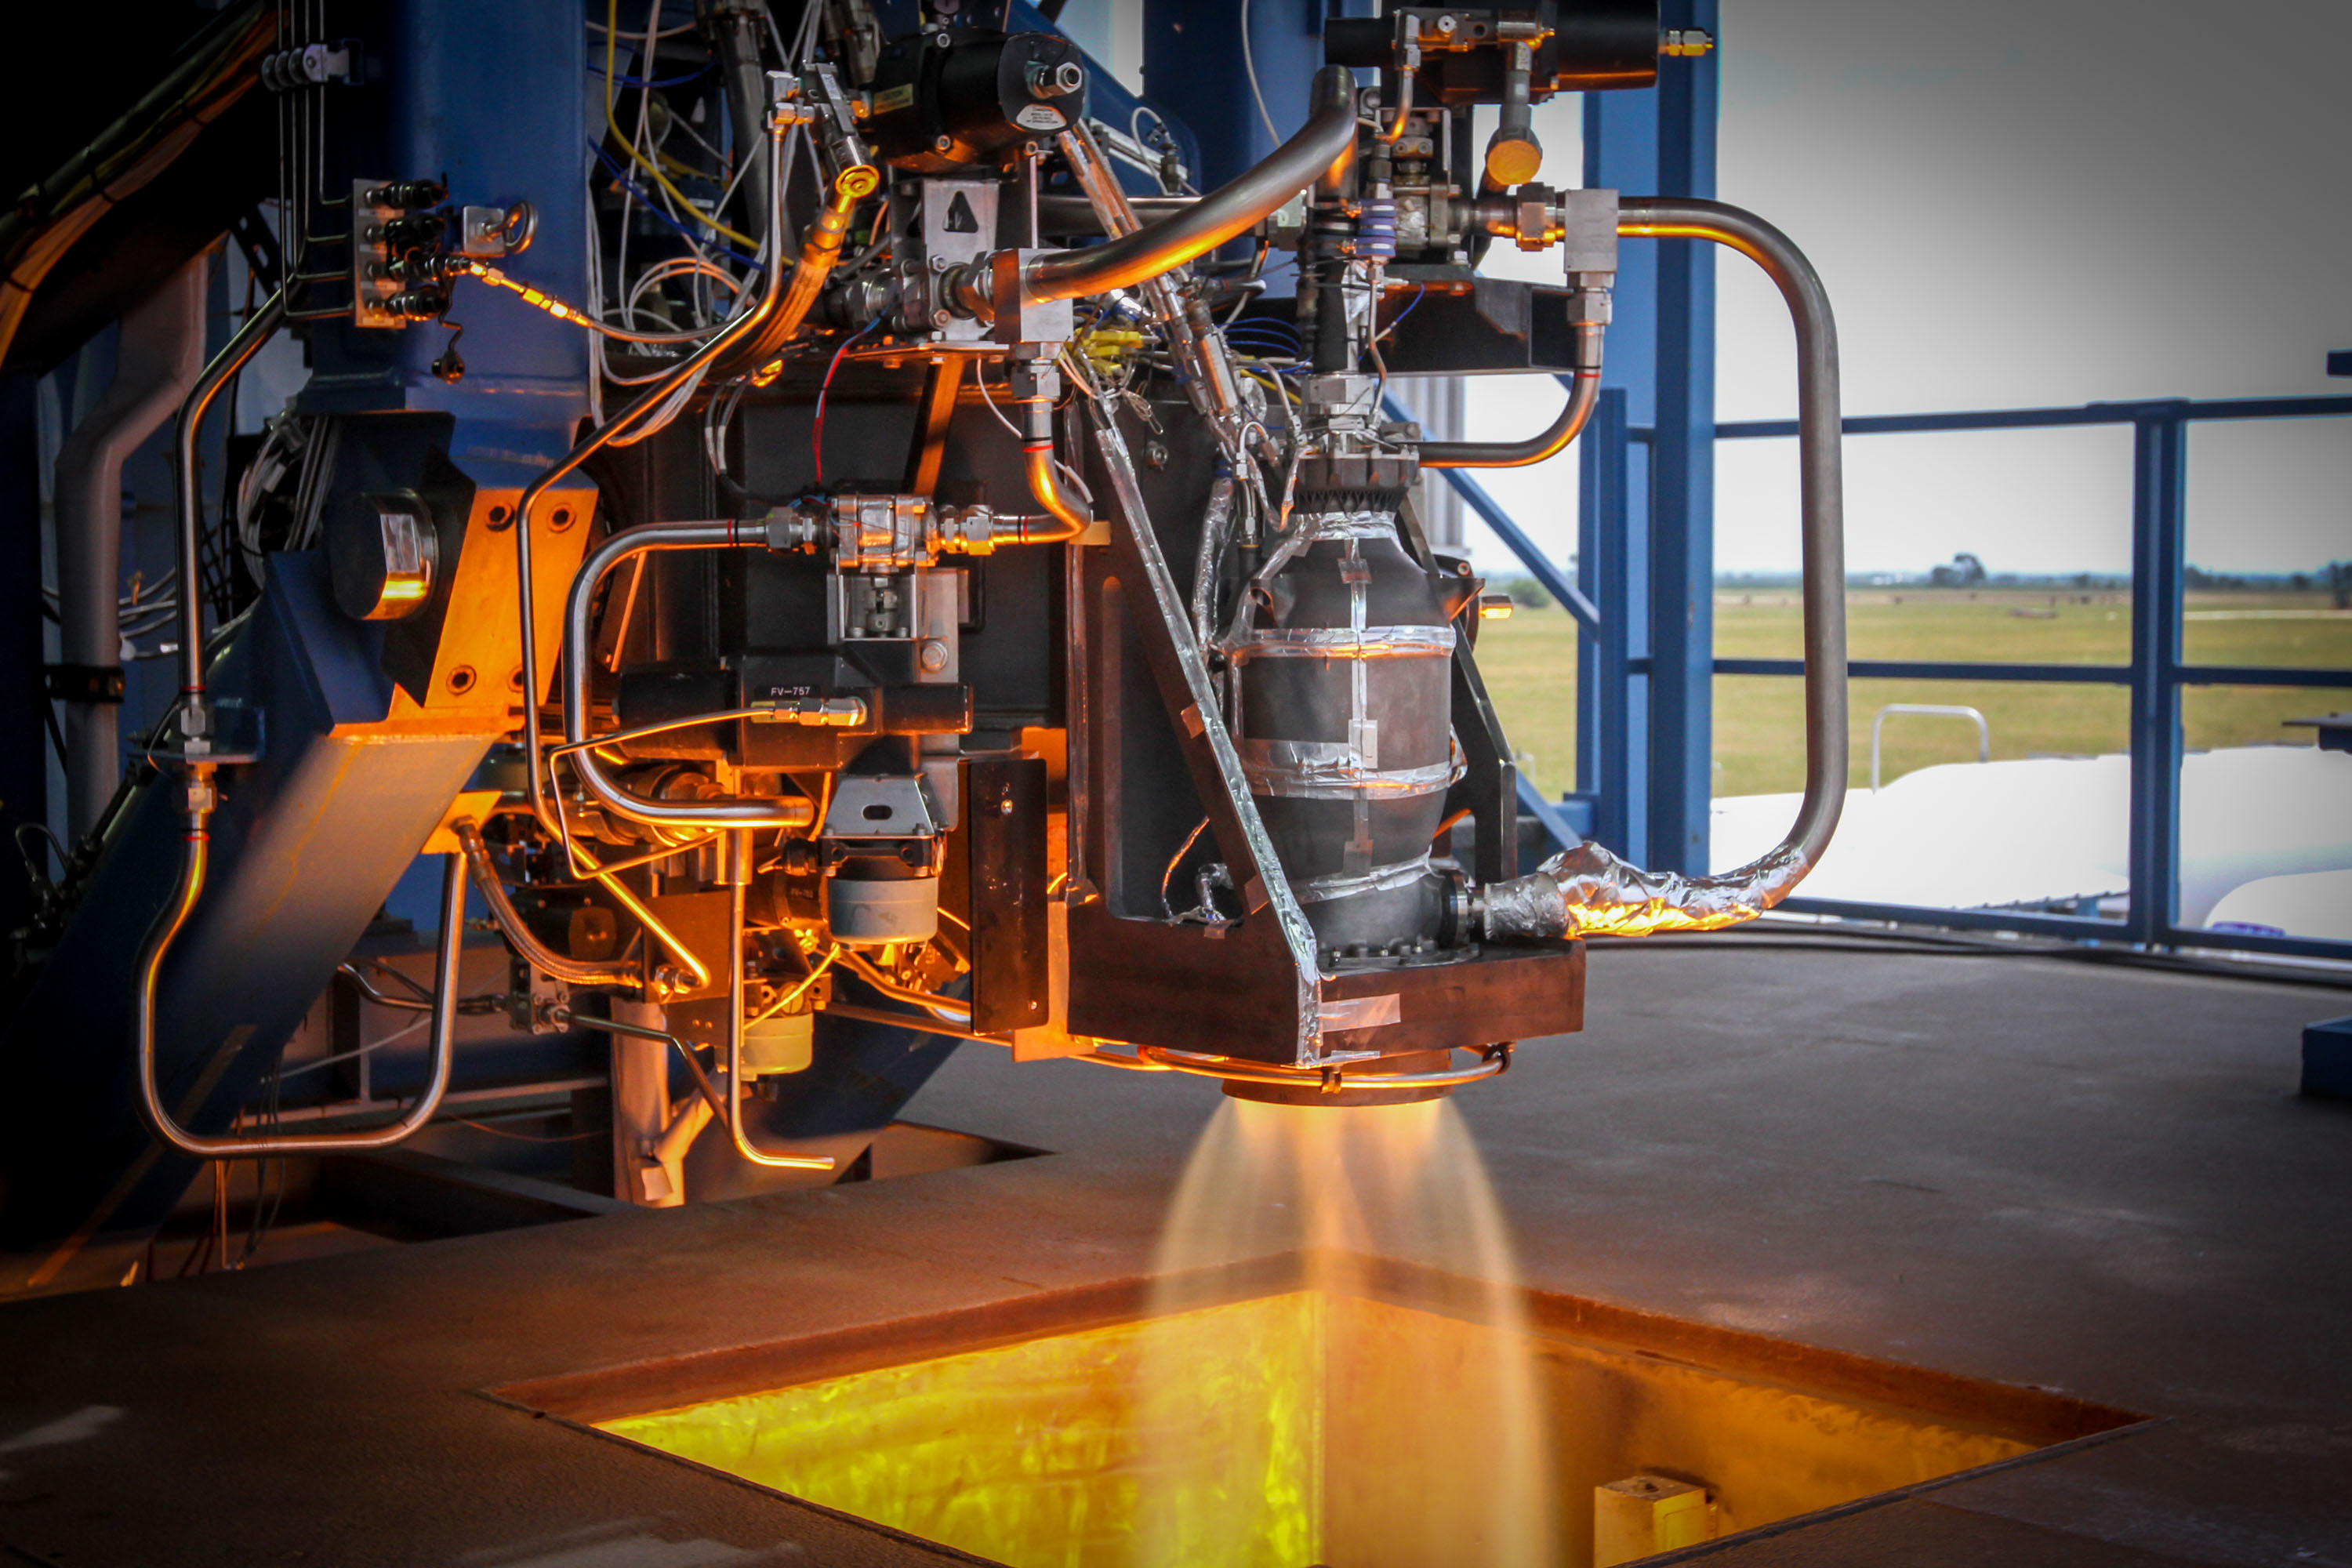
\includegraphics[height=4.5cm]{superdraco.jpg}}
    \hfil
    \subfloat[][A conventional hinge is seen in the background and a 3D-printed metal hinge is seen in the foreground - EADS.]{\label{fig:EADS_hinge}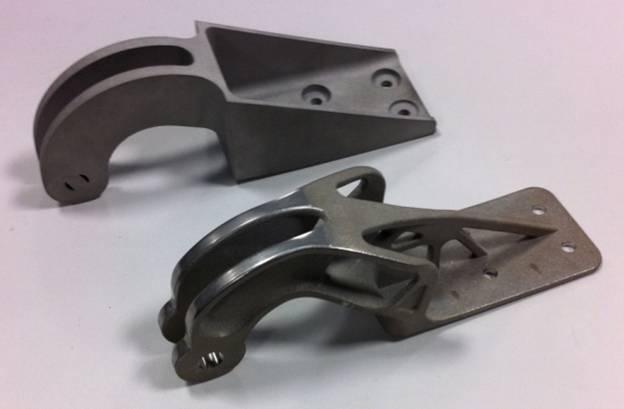
\includegraphics[height=4.5cm]{EADS_3D_printed_hinge.jpg}}
    \caption{Thanks to its particular properties, 3D printing is hitting the industry}
    \label{fig:3D_printed_objects}
\end{figure}

The SuperDraco (see \figurename~\ref{fig:superdraco}) differs from most rocket engines in that its combustion chamber is 3D printed by direct metal laser sintering (DMLS), where complex metal structures are printed by using a laser to build the object out of metal powders one thin layer at a time. The regeneratively-cooled combustion chamber is made of inconel; a family of nickel-chromium alloy that is notable for its high strength and toughness.

\begin{quotation}
    Through 3D printing, robust and high-performing engine parts can be created at a fraction of the cost and time of traditional manufacturing methods. SpaceX is pushing the boundaries of what additive manufacturing can do in the 21st century, ultimately making our vehicles more efficient, reliable and robust than ever before.
    \signed{Elon Musk, SpaceX CEO/CTO and Tesla Motors CEO.}
\end{quotation}


Parts for cars and satellites can be optimised to be lighter and - simultaneously - incredibly robust.

The AMAZE project has been able to print airplane wing sections as well as jet engine parts, and the ESA hopes to one day print a satellite as one piece:
\begin{quotation}
    This novel technology offers many advantages. 3D printing, formally known as additive manufacturing, can create complex shapes that are impossible to manufacture with traditional casting and machining techniques. Little to no material is wasted and cutting the number of steps in a manufacturing chain offers enormous cost benefits.
    \signed{European Space Agency (ESA)}
\end{quotation}




\subsection{Conclusion} % (fold)

3D printers open new horizons as they are able to produce parts which were, until now, either not possible or extremely expensive to produce using classical techniques while adding several key abilities:
\begin{itemize}
    \item \textbf{Accessible:} 3D printed part can be obtained everywhere, either by personal printing or by using web service\footnote{examples: i.materialise, shapeways or sclupteo}.
    \item \textbf{Low cost:}  from few dozens of cents if produced on personal printer to few dozens of euros if outsourced through web services. Also the cost is not proportional to the part complexity, meaning designers are free to explore the shape they want with almost no constraints.
    \item \textbf{Fast:} The production took only few hours from scratch and does not require any specific upfront tooling.
    \item \textbf{Skill-free:} while the production process is fully numerical, few or no special skills is required.
    \item \textbf{Multi-material, precise and robust:} the current 3D printers can create precise (up to 0.1mm) part in different materials such as Polyamide, PLA, ABS and even titanium or flexible material. The obtained parts are robust and can often be used as final parts for several years.
    \item \textbf{Reduces the number of part:} 3D printing permits to print complex part and even assembled parts as complex as bearing or gearbox. This means we can replace multiple parts that have to be assembled by a unique one ready-to-use right after its production.
\end{itemize}



The cost depends on the size and not on the complexity of the part meaning we can freely optimize the shape.


\newpage
\section{The open hardware movement} % (fold)

The concept of "open-source hardware" or "open hardware" is not as well known or widespread as the free software or open-source software concept yet. However, it shares the same principles: anyone should be able to see the source (the design documentation in case of hardware), study it, modify it and share it.

The emergence of new and accessible rapid prototyping techniques change the way to produce things. Because it is now quick, simple and cheap to make things, it opens the realm of possibility to share hardware because anyone can produce it. Open source hardware is now making sense and is currently exponentially growing.

In this section, we will ...

\subsection{Open hardware in the industrial history.} % (fold)

In the 18th century, London and Lyon(France) are two majors silk manufacturer town. Because London is on the way to take the leadership, Lyon try an new and original politic for innovation. They decide to freely diffuse the novel technique. Inventors are invited in the city hall to present publicly their innovations. They are then rewarded a first time for the presentation and a second time when the innovation is actually implemented on Lyon machines. Follows this politic, decades of cumulative innovations such as: perforated paper tape (1725 B.Bouchon), punched card program (1728, J-B.Falcon), the Jacquard loom (1801, J-M. Jacquard), sewing machine (1829, B.Thimonnier). Meanwhile, silk production in London is governed by patents, technique are kept secret and monopolized by theirs inventors. \cite{alain1997fate}

The impact of this two opposed political choices turn largely in the advantage for Lyon. In 1815, Lyon had 14500 looms and London 12000. But in 1853, Lyon had 60000 looms while London fell to only 5000. London become a silk importer.

Lyon stimulates inventions and disseminates innovation: looms become programmable, agile order processing and production, standardization of parts, appearance counter-tops parts, services grow, the Lyon looms park is up to date and operational.
In London, the industry is controlled by investors, customers must order large series, the choice decreases, the period is longer, the artisans become employees, wages fall and Londoner park looms state is deteriorated.

The Lyon politic has created a win-win ecosystem creating both jobs opportunity and advanced technology. Thanks to this choice, the city took the leadership over London.

\subsection{Open Hardware definition} % (fold)

The Open Source Hardware Association (OSHWA) aims to be the voice of the open hardware community. It promotes the use and development of open source hardware for education and economic development, collect, compile and publish data on the open source movement and organize the movement around shared and principles.

Also the Open Source Hardware Association defines\footnote{Complete definition available on \url{http://www.oshwa.org/definition/}.} the open source hardware as:

\begin{row}{4}{2}
    \begin{cell}{3}
        \emph{Hardware whose design is made publicly available so that anyone can study, modify, distribute, make, and sell the design or hardware based on that design. The hardware’s source, the design from which it is made, is available in the preferred format for making modifications to it. Ideally, open source hardware uses readily-available components and materials, standard processes, open infrastructure, unrestricted content, and open-source design tools to maximize the ability of individuals to make and use hardware. Open source hardware gives people the freedom to control their technology while sharing knowledge and encouraging commerce through the open exchange of designs.}
    \end{cell}
    \begin{cell}{1}
        \begin{NFfigure}
            \centering
                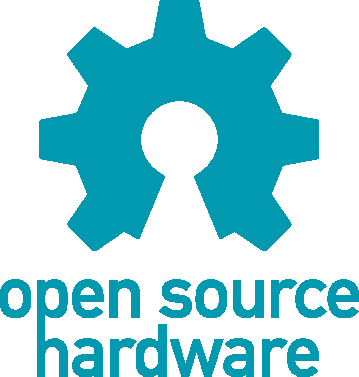
\includegraphics[height=4cm]{oshw-logo.pdf}
            \caption{The open source hardware logo}
            \label{fig:ohw-logo}
        \end{NFfigure}
    \end{cell}
\end{row}


\subsection{Open source hardware licenses} % (fold)

The Open Source Hardware Association definition is not enough, a legal framework is needed to both protect and promote open hardware project. This is the role of the open source licenses which will be discussed in this section.

In general, there are two broad classes of open-source licenses: copyleft and permissive. Copyleft licenses (sometimes referred to as “viral”) are those which require derivative works to be released under the same license as the original; common copyleft licenses include the GNU General Public License (GPL) and the Creative Commons Attribution-ShareAlike license. Other copyleft licenses have been specifically designed for hardware; they include the CERN Open Hardware License (OHL) and the TAPR Open Hardware License (OHL). Permissive licenses are those which allow for proprietary (closed) derivatives; they include the FreeBSD license, the MIT license, and the Creative Commons Attribution license


\subsubsection{Creative Commons licenses} % (fold)
\begin{row}{4}{2}
    \begin{cell}{3}
        Founded in 2001, Creative Commons is a nonprofit organization that enables the sharing and use of creativity and knowledge through free legal tools. They provide a free and understandable licenses standardizing the way to share and use creative work. Thanks to the use of several modules which can be combined, the Creative Commons licenses permit to the creator to modify his copyright terms to best suit his needs. First intended for artistic and cultural content such as music and writing, the Creative Commons are now used also to share open source hardware files.
    \end{cell}
    \begin{cell}{1}
        \begin{NFfigure}
            \centering
                
\includegraphics[height=3cm]{cc-logo.png}
            \caption{Creative Commons logo}
            \label{fig:cc_logo}
        \end{NFfigure}
    \end{cell}
\end{row}
The Creative Commons licenses are based on four major condition modules:
\begin{description}
    \item[Attribution (BY)]: requiring attribution to the original author.
    \item[Non Commercial (NC)]: requiring the work is not used for commercial purposes
    \item[No Derivative works (ND)]: allowing only the original work, without derivatives
    \item[Share Alike (SA)]: allowing derivative works under the same or a similar license (later or jurisdiction version).
\end{description}


The combination of these modules leads to six licenses (see \figurename~\ref{fig:all-cc-licenses}) but related to the open only two of them are considered as open source following the OSHW definition:
\begin{description}
    \item[Attribution CC BY] People can distribute, remix, tweak and build upon the licensed work, even commercially, as long as they credit the authors of the original creation.
    \item[Attribution-ShareAlike CC BY-SA] People can distribute, remix, tweak and build upon the licensed work, even commercially, as long as they credit the authors and license their new creations under the identical terms. \textbf{This license is often compared to “copyleft” free and open source software licenses.}
\end{description}

\begin{figure}[]
    \begin{center}
        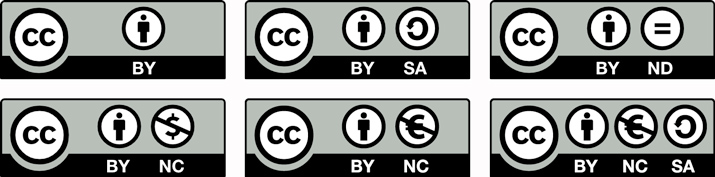
\includegraphics[width=0.8\linewidth]{all-cc-licenses.jpg}
    \end{center}
    \caption{The combination of the 4 Creative Commons modules give 6 licenses allowing creators to choose how they want to share their work and how "open" they are.}
    \label{fig:all-cc-licenses}
\end{figure}

\subsubsection{CERN OHL} % (fold)

Inspired by the open source software movement, the Open Hardware Repository\footnote{\url{http://www.ohwr.org/}} was created to enable hardware developers to share the results of their R\&D activities. The recently published (mars 2013) CERN Open Hardware Licence offers the legal framework to support this knowledge and technology exchange.

The CERN–OHL is to hardware what the General Public Licence (GPL) is to software. It defines the conditions under which a licensee will be able to use or modify the licensed material and is compliant with the OSHWA definition criteria. In the spirit of knowledge sharing and dissemination, the CERN Open Hardware Licence (CERN OHL) governs the use, copying, modification and distribution of hardware design documentation, and the manufacture and distribution of products\footnote{License details available on \url{http://www.ohwr.org/projects/cernohl/wiki}}.


\subsubsection{TAPR Open Hardware License (OHL)}
Specifically designed for open hardware, and avoids the issues other licenses have with focusing on copyright protecting documentation instead of the right to make, distribute, or use a product based on that documentation. Requires that all derived works use the same license and include before and after documentation if any changes were made.

Visit the TAPR website for the full text of the TAPR Open Hardware License (OHL). The numbered sections of the agreement take precedence over this preamble.


\subsection{Some famous open hardware projects} % (fold)

Based on the open source hardware philosophy, several company and project have been created over the past ten years (see \figurename~\ref{fig:oh_evolution}).

\begin{figure}[h]
\centering
    \subfloat[][Creation of new open hardware project per year between 2005 and 2011.]{\label{fig:oh_project_evolution}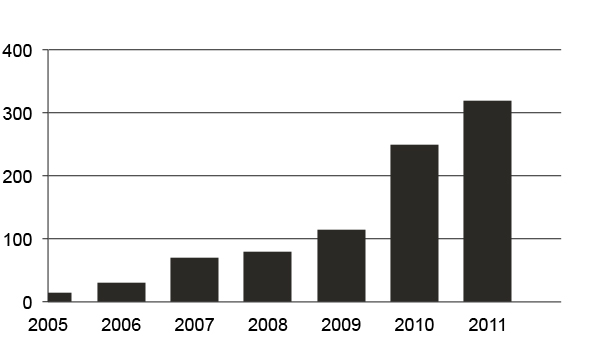
\includegraphics[width=0.45\linewidth]{oh_project_evolution.jpg}}
    \hfil
    \subfloat[][Start-up creation based on open hardware distribution]{\label{fig:oh_startup_creation}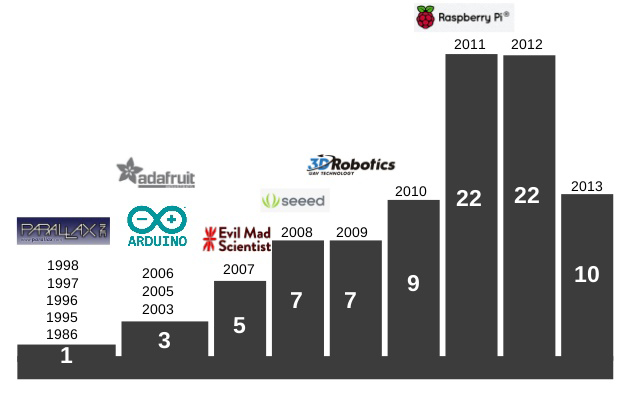
\includegraphics[width=0.45\linewidth]{oh_startup_creation.jpg}}
    \caption{Evolution of the open source hardware movement in the past decades.Graphic extracted from \emph{HOPE 2010 - How to run an open source hardware company}}
    \label{fig:oh_evolution}
\end{figure}


Several kind of object begin to have an open source version even the most advanced ones such as laptop (Novena project\footnote{\url{https://www.crowdsupply.com/kosagi/novena-open-laptop}}), reflex camera (OpenReflex\footnote{\url{http://www.instructables.com/id/3D-Printed-Camera-OpenReflex/}}) or even car (LocalMotors\footnote{\url{https://localmotors.com/vehicles/}}, OSVehicle\footnote{\url{http://www.osvehicle.com/}}).

Yet we will keep project in the scope of the personal production and

\subsubsection{Arduino} % (fold)

Students from the Interaction Design Institute Ivrea in Italy were using \emph{BASIC Stamp}\footnote{A BASIC Stamp module is a single-board computer that runs the Parallax PBASIC language interpreter in its microcontroller.} for a cost of \$100.

\begin{row}{4}{2}
    \begin{cell}{3}
      Started in 2005 by Banzi and al., the Arduino project aimed to offer an affordable and easy to use electronics board for student-friendly price: \$30. The first wiring design was done during the phd thesis of Hernando Barragan~\cite{barragan2004wiring}. After the wiring platform was complete, researchers worked to make it lighter, less expensive, and available to the open source community.
    \end{cell}
    \begin{cell}{1}
        \begin{NFfigure}
            \centering
                
\includegraphics[height=2.5cm]{arduino_logo.png}
            \caption{The Arduino logo}
            \label{fig:arduino_logo}
        \end{NFfigure}
    \end{cell}
\end{row}

\begin{quotation}
  Arduino is a platform for prototyping interactive objects using electronics. It consists of both hardware and software: a circuit board that can be purchased at low cost or assembled from freely-available plans; and an open-source development environment and library for writing code to control the board. Arduino comes from a philosophy of learning by doing and strives to make it easy to work directly with the medium of interactivity. It extends the principles of open source to the realm of hardware, supporting a community of people working with and extending the platform. It has been used in universities around the world and in numerous works of interactive art.

  \signed{Mellis~\cite{mellis2007arduino}}
\end{quotation}

The arduino story was one of the first hardware project with a real desire to promote the innovation trough open source, to make it work they had to find an appropriate licensing solution that could apply to their board. After some investigation, they realized that if they simply looked at their project differently, (i.e. considering the source files as documentation\footnote{\emph{"You could think of hardware as piece of culture you want to share with other people"}, Banzi. }), they could use a license from Creative Commons normally used for cultural works such as music and writing.

Today, Arduino is a very successful project. The boards and derivatives are used by hundreds of thousands people and a lot of project from all domains would not possible if Arduino have not existed, among them Poppy.

\subsubsection{Shapeoko}

\begin{figure}[!h]
    \begin{center}
        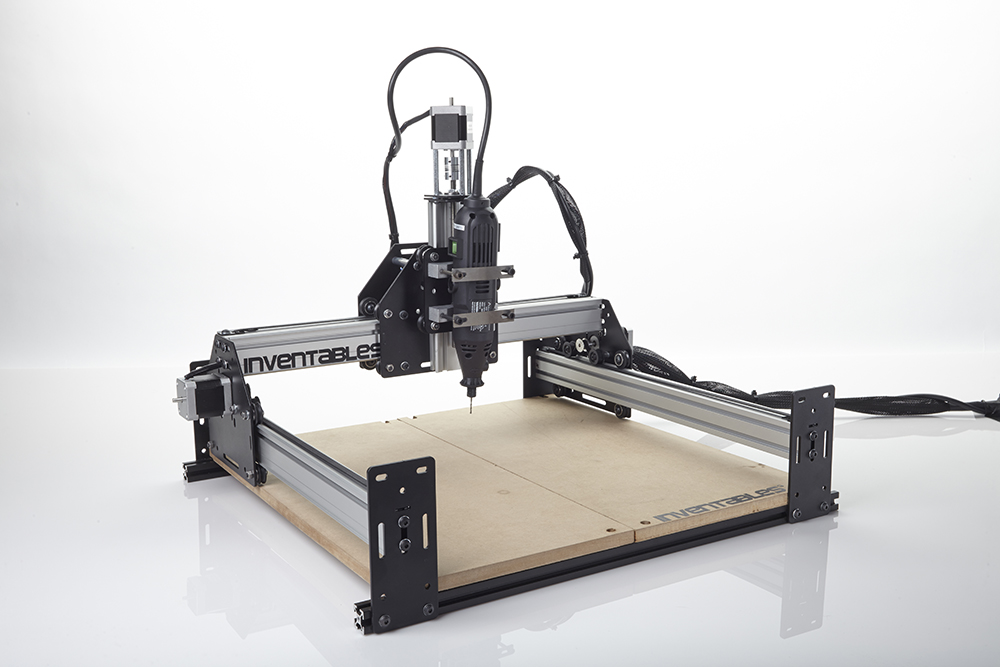
\includegraphics[width=0.8\linewidth]{shapeoko_v2.jpg}
    \end{center}
    \caption{The shapeoko v2 is a low cost and open source CNC 2.5 axes.}
    \label{fig:shapeoko}
\end{figure}

Designed by Edward Ford, Shapeoko (see \figurename~\ref{fig:shapeoko}) is a simple, low cost (\$685) and open source (CC BY-SA)CNC milling machine. It is based on two other open hardware projects: MakerSlide\footnote{Open source linear bearing system under Creative Common BY-SA licenses: \url{http://makerslide.com/}} for linear motion and an Arduino board for the control.



\subsubsection{RepRap} % (fold)

The RepRap project started in 2005 and based on the Fab@Home\footnote{\url{http://www.fabathome.org/}} principles, developped a multi-proposed open source 3D printer using Fused Deposition Modeling\footnote{TODO}(FFD) technique with the particularity to be largerly self-replicating:

\begin{quotation}
    RepRap is an open-source self-replicating rapid prototyping machine. It is a robot that uses fused-filament fabrication1 to make engineering components and other products from a variety of thermoplastic polymers. RepRap has been designed to be able automatically to print out a significant fraction of its own parts. All its remaining parts have been selected to be standard engineering materials and components available cheaply worldwide. As the machine is free and open-source anyone may – without royalty payments – make any number of copies of it ether for themselves or for others, using RepRap machines themselves to reproduce those copies.

    \signed{~\cite{jones2011reprap}}
\end{quotation}


\begin{figure}[]
\centering
    \subfloat[][RepRap v2]{\label{fig:RepRap_v2}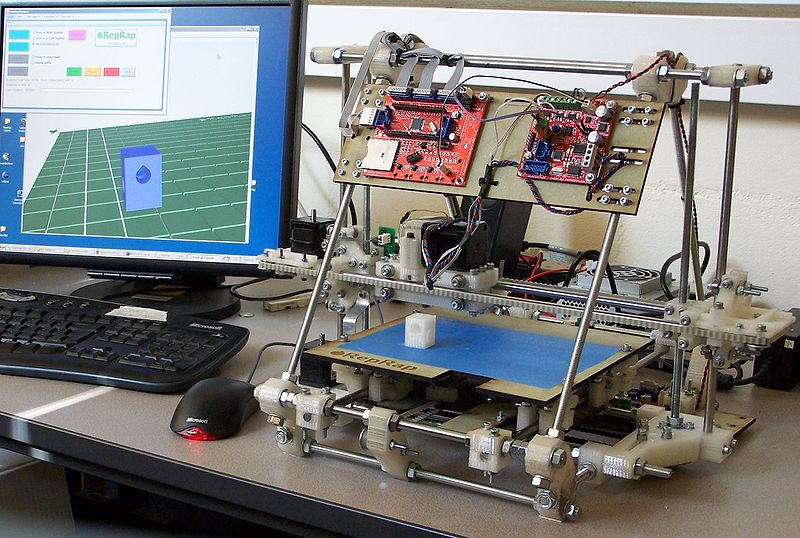
\includegraphics[width=0.45\linewidth]{RepRap_v2.jpg}}
    \hfil
    \subfloat[][MakerBot Replicator v1]{\label{fig:makerbot-replicator}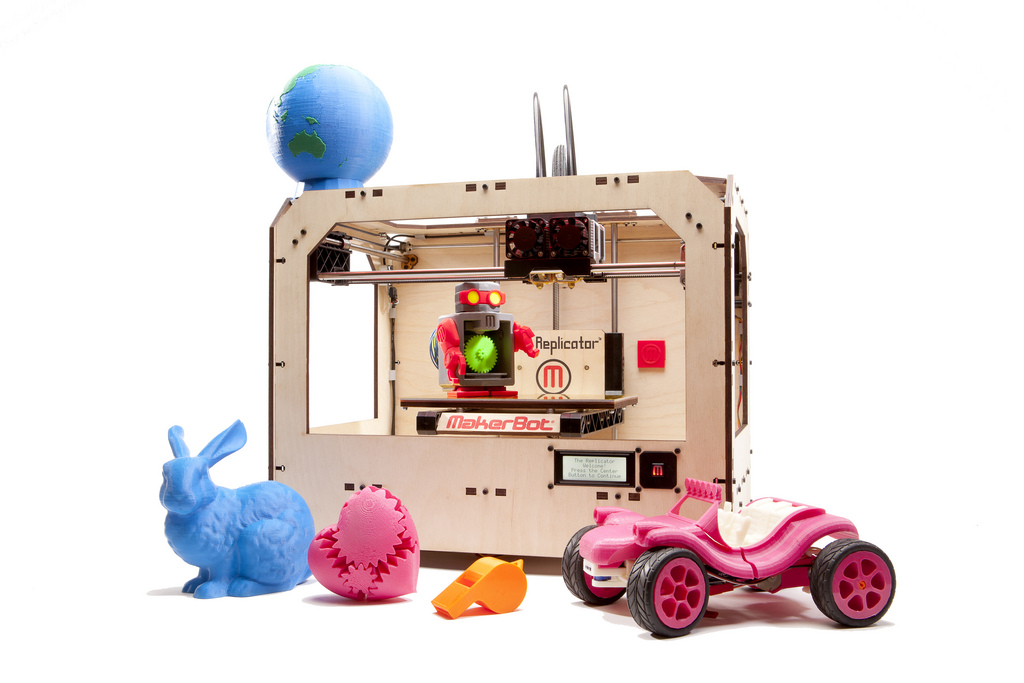
\includegraphics[width=0.45\linewidth]{makerbot-replicator.jpg}}
    \caption{}
    \label{fig:RepRap_project}
\end{figure}


Distributed under GNU General Public License, the RepRap (see \figurename~\ref{fig:RepRap_v2}) was one of the first low-cost 3D printer. The fact it is genuinely collaborative, this project generated a so large number of variations and interpretations that is even difficult to count (see \figurename~\ref{fig:RepRap_family_tree}). One of them is the now famous Makerbot Replicator (see \figurename~\ref{fig:makerbot-replicator}). Now Makerbot is one of the major worldwide general public 3D printer distributor.
